% Overshoot: manuscript draft for European Journal of Physics.
% Written with the standard article class and IOP's numeric bibliography style (iopart-num);
% move to the IOP iopart template before submission.
\documentclass[11pt,a4paper]{article}
\usepackage[T1]{fontenc}
\usepackage[utf8]{inputenc}
\usepackage{lmodern}
\usepackage[margin=2.4cm]{geometry}
\usepackage{amsmath,amssymb}
\usepackage{graphicx}
\usepackage{booktabs}
\usepackage{siunitx}
\usepackage{caption}
\usepackage[hidelinks]{hyperref}
\usepackage{xurl}
\captionsetup{font=small,labelfont=bf}
\sisetup{per-mode=symbol,group-separator={\,}}
\newcommand{\IKr}{I_{\mathrm{Kr}}}
\newcommand{\IKs}{I_{\mathrm{Ks}}}
\newcommand{\ICaL}{I_{\mathrm{CaL}}}
\newcommand{\INa}{I_{\mathrm{Na}}}
\newcommand{\etal}{\textit{et al}}

\title{Overshoot: a browser game for learning how ion channels\\ shape action potentials and the electrocardiogram}
\author{Toni Giorgino\\[2pt]
\small Istituto di Biofisica, Consiglio Nazionale delle Ricerche (IBF-CNR), Italy\\
\small \texttt{toni.giorgino@cnr.it}}
\date{}

\begin{document}
\maketitle

\begin{abstract}
\noindent Conductance-based models of excitable membranes are a showcase of quantitative physics in biology: a capacitor, a handful of nonlinear voltage-dependent conductances and their Nernst batteries reproduce the shape of a nerve impulse or a cardiac action potential. Students usually meet these models in the forward direction, integrating given equations. We describe \emph{Overshoot}, a free browser game that poses the inverse problem. Each level shows a target recording, and the player adjusts the density of each ion-channel type until a simulated cell, or a strip of ventricular wall, reproduces it. The nine levels run from the Hodgkin--Huxley squid axon through cortical and thalamic neurons to human ventricular myocytes, a transmural pseudo-electrocardiogram and a drug-safety puzzle. All targets are generated by published models with unmodified equations. Scoring follows how modellers fit data, comparing electrophysiological features within physical tolerances. A slow-motion ``magnifying lens'' shows ions crossing the membrane at a calibrated rate, so the number of dots that cross equals the true number of ions moved. We present the physics, the game design, a set of quantitative checks against physiology, and suggested classroom exercises on degeneracy, charge balance and the origin of the T wave.
\end{abstract}

\section{Introduction}

The Hodgkin--Huxley (HH) model \cite{HH1952} is one of the great successes of physical modelling in biology. Treating the membrane as a capacitor in parallel with voltage-gated conductances, Hodgkin and Huxley fitted their voltage-clamp data and then \emph{predicted} the shape, propagation speed and refractoriness of the nerve impulse. The same formalism, extended to a few dozen currents and intracellular ion concentrations, now describes human ventricular myocytes \cite{TNNP2004,OHara2011}. It underpins regulatory drug-safety testing \cite{Colatsky2016}.

In physics and biophysics courses the model usually appears as a set of ordinary differential equations to integrate. That direction teaches numerics but hides the question experimentalists and modellers actually face: \emph{given a recording, which channels, and how many of each, produce it?} The inverse problem exposes the physics more sharply. The player must reason about time constants, reversal potentials and the balance of inward and outward currents. It also exposes a deep and slightly uncomfortable fact: different channel mixtures can produce nearly identical waveforms \cite{Prinz2004,MarderGoaillard2006}.

\emph{Overshoot} turns this inverse problem into a game, in the sense of using game design elements in a non-game context \cite{Deterding2011}. The game takes its name from the part of the action potential that rises above \SI{0}{\milli\volt}. Each level presents a target trace and a ``channel rack'' of sliders, scores the match, and rewards it with up to three stars. It runs entirely in a web browser, as a single self-contained HTML file with no installation and no server. Research simulators such as NEURON \cite{HinesCarnevale1997} and Myokit \cite{Clerx2016} are general-purpose environments. Overshoot instead aims for a short path from curiosity to insight: one idea per level, physical units throughout, and the physiology explained only after the player has struggled with it.

This paper describes the models (section~\ref{sec:models}), the game mechanics (section~\ref{sec:game}), the calibrated slow-motion view of ion fluxes (section~\ref{sec:lens}), quantitative checks (section~\ref{sec:checks}) and classroom uses (section~\ref{sec:class}). It ends with the limitations (section~\ref{sec:limits}). The game is available at \url{https://tonigi.github.io/overshoot-game/}, and the source code at \url{https://github.com/tonigi/overshoot-game}, under the Apache 2.0 licence.

\section{Physical models}\label{sec:models}

\subsection{Membrane equation}
Every single-cell level integrates the current-balance equation of a patch of membrane,
\begin{equation}
C_m \frac{\mathrm{d}V}{\mathrm{d}t} = -\sum_k \bar g_k \, \prod_j x_{kj}^{p_{kj}} \,(V - E_k) \; - \; I_{\mathrm{pump}} - I_{\mathrm{exch}} + I_{\mathrm{stim}}(t),
\label{eq:membrane}
\end{equation}
where $\bar g_k$ is the maximal conductance of channel type $k$ and $E_k$ its reversal potential. Each gate $x$ relaxes towards a voltage-dependent steady state,
$\mathrm{d}x/\mathrm{d}t = \left(x_\infty(V)-x\right)/\tau_x(V)$.
The cardiac model adds electrogenic transport by the Na$^+$/K$^+$ pump and the Na$^+$/Ca$^{2+}$ exchanger (NCX), plus intracellular Ca$^{2+}$ handling, which feeds back on $\ICaL$ and NCX. The maximal conductance is proportional to the number of channels per unit area, $\bar g_k = n_k \gamma_k$, where $\gamma_k$ is the single-channel conductance. Changing $\bar g_k$ is therefore changing \emph{channel density}, and this is the player's control.

\subsection{Models used}
The targets come from three published models with unmodified equations (table~\ref{tab:levels}).
\begin{itemize}
\item The 1952 HH squid axon \cite{HH1952}, at \SI{6.3}{\celsius}.
\item Two minimal neocortical and thalamic models by Pospischil \etal\ \cite{Pospischil2008}. The regular-spiking pyramidal cell uses Na$^+$, delayed-rectifier K$^+$, slow Kv7 (M-current \cite{BrownAdams1980}) and leak conductances. The thalamic cell replaces the M-current with a T-type Ca$^{2+}$ current, which produces rebound bursts.
\item The human ventricular model of ten Tusscher, Noble, Noble and Panfilov (TNNP 2004) \cite{TNNP2004}: 17 state variables, 12 membrane currents, and sarcoplasmic-reticulum Ca$^{2+}$ release.
\end{itemize}
Levels change parameters, never equations. The single exception, discussed below, is an epicardial $\IKs$ density taken from the authors' 2006 revision \cite{TP2006}.

\begin{table}[t]
\centering\small
\caption{The nine levels. \emph{Start} is the score of the initial slider settings against the target. One star requires 70\%.}
\label{tab:levels}
\begin{tabular}{@{}rlllr@{}}
\toprule
\# & Level & Model & Adjustable quantities & Start \\
\midrule
1 & Squid giant axon & HH 1952 & $\bar g_{\mathrm{Na}}, \bar g_{\mathrm{K}}, \bar g_{\mathrm{L}}$ & 15\% \\
2 & Pyramidal neuron (adaptation) & Pospischil 2008 & Nav, Kv2, Kv7, leak & 32\% \\
3 & Thalamic neuron (rebound burst) & Pospischil 2008 & Nav, Kv2, Cav3.1, leak & 18\% \\
4 & Ventricular myocyte, epicardium & TNNP 2004 & six channels & 46\% \\
5 & Mid-myocardial M cell & TNNP 2004 & six channels & 62\% \\
6 & Mystery patient (long QT) & TNNP 2004 & six channels & 40\% \\
7 & Electrolyte emergency & TNNP 2004 & $[\mathrm{K}^+]_o, [\mathrm{Na}^+]_o, [\mathrm{Ca}^{2+}]_o$ & 8\% \\
8 & The T wave & 1D TNNP strand & coupling, $\IKs$ per layer, $I_{\mathrm{to}}$, $\IKr$ & 47\% \\
9 & The hERG paradox & 1D TNNP strand & remaining $\ICaL, \INa, \IKs, I_{\mathrm{K1}}$ & 43\% \\
\bottomrule
\end{tabular}
\end{table}

\subsection{Tissue and the pseudo-ECG}
The electrocardiogram (ECG) is not the voltage of any cell. It is the extracellular field of many cells activating and recovering at slightly different times. Levels 8 and 9 couple 60 TNNP cells in a \SI{1.2}{\centi\metre} strand spanning the left-ventricular wall. Following the monodomain cable equation,
\begin{equation}
\frac{\partial V}{\partial t} = D\,\frac{\partial^2 V}{\partial x^2} - \frac{I_{\mathrm{ion}}(V,\mathbf{y})}{C_m},
\end{equation}
the strand is stimulated at the endocardial end. The inner 25\% has endocardial properties, the middle 35\% mid-myocardial ``M cell'' properties \cite{SicouriAntzelevitch1991}, and the outer 40\% epicardial properties. The pseudo-ECG at a point $x'$ on the strand axis, \SI{2}{\centi\metre} beyond the epicardium, is \cite{GimaRudy2002}
\begin{equation}
\phi_e(x') = \frac{a^2\sigma_i}{4\sigma_e}\int \left(-\frac{\partial V}{\partial x}\right)\frac{\partial}{\partial x}\!\left(\frac{1}{r}\right)\mathrm{d}x, \qquad r = |x - x'|,
\label{eq:pseudoecg}
\end{equation}
normalised so that the reference QRS complex has unit amplitude. Equation~(\ref{eq:pseudoecg}) is the key teaching point: only voltage \emph{gradients} along the wall produce a signal. During the QRS the gradient is the activation front, so the QRS width is the transmural conduction time, set by the gap-junction coupling $D$. During the T wave the gradient comes from cells repolarising at different times.

\subsection{Numerics and speed}
Gates are advanced with the Rush--Larsen exponential integrator \cite{RushLarsen1978},
$x(t+\Delta t) = x_\infty + (x - x_\infty)\,e^{-\Delta t/\tau_x}$. Voltage and concentrations use forward Euler. The cardiac time step is \SI{0.01}{\milli\second} during the upstroke and \SI{0.05}{\milli\second} elsewhere. The strand uses $\Delta x = \SI{0.2}{\milli\metre}$, with $D\Delta t/\Delta x^2 \le 0.09$, well inside the explicit stability limit.

Interactivity sets the budget. A single-cell simulation must finish in about \SI{40}{\milli\second} so the trace follows the slider. Two paced beats from a precomputed \SI{1}{\hertz} steady state, with intracellular Na$^+$ and K$^+$ held fixed, take about \SI{35}{\milli\second} in a current browser. A strand simulation takes about \SI{0.7}{\second} and runs in a background Web Worker. While it runs, a ``Simulating\ldots'' indicator is shown, and only the latest slider position is simulated next.

\section{Game design}\label{sec:game}

\begin{figure}[t]
\centering
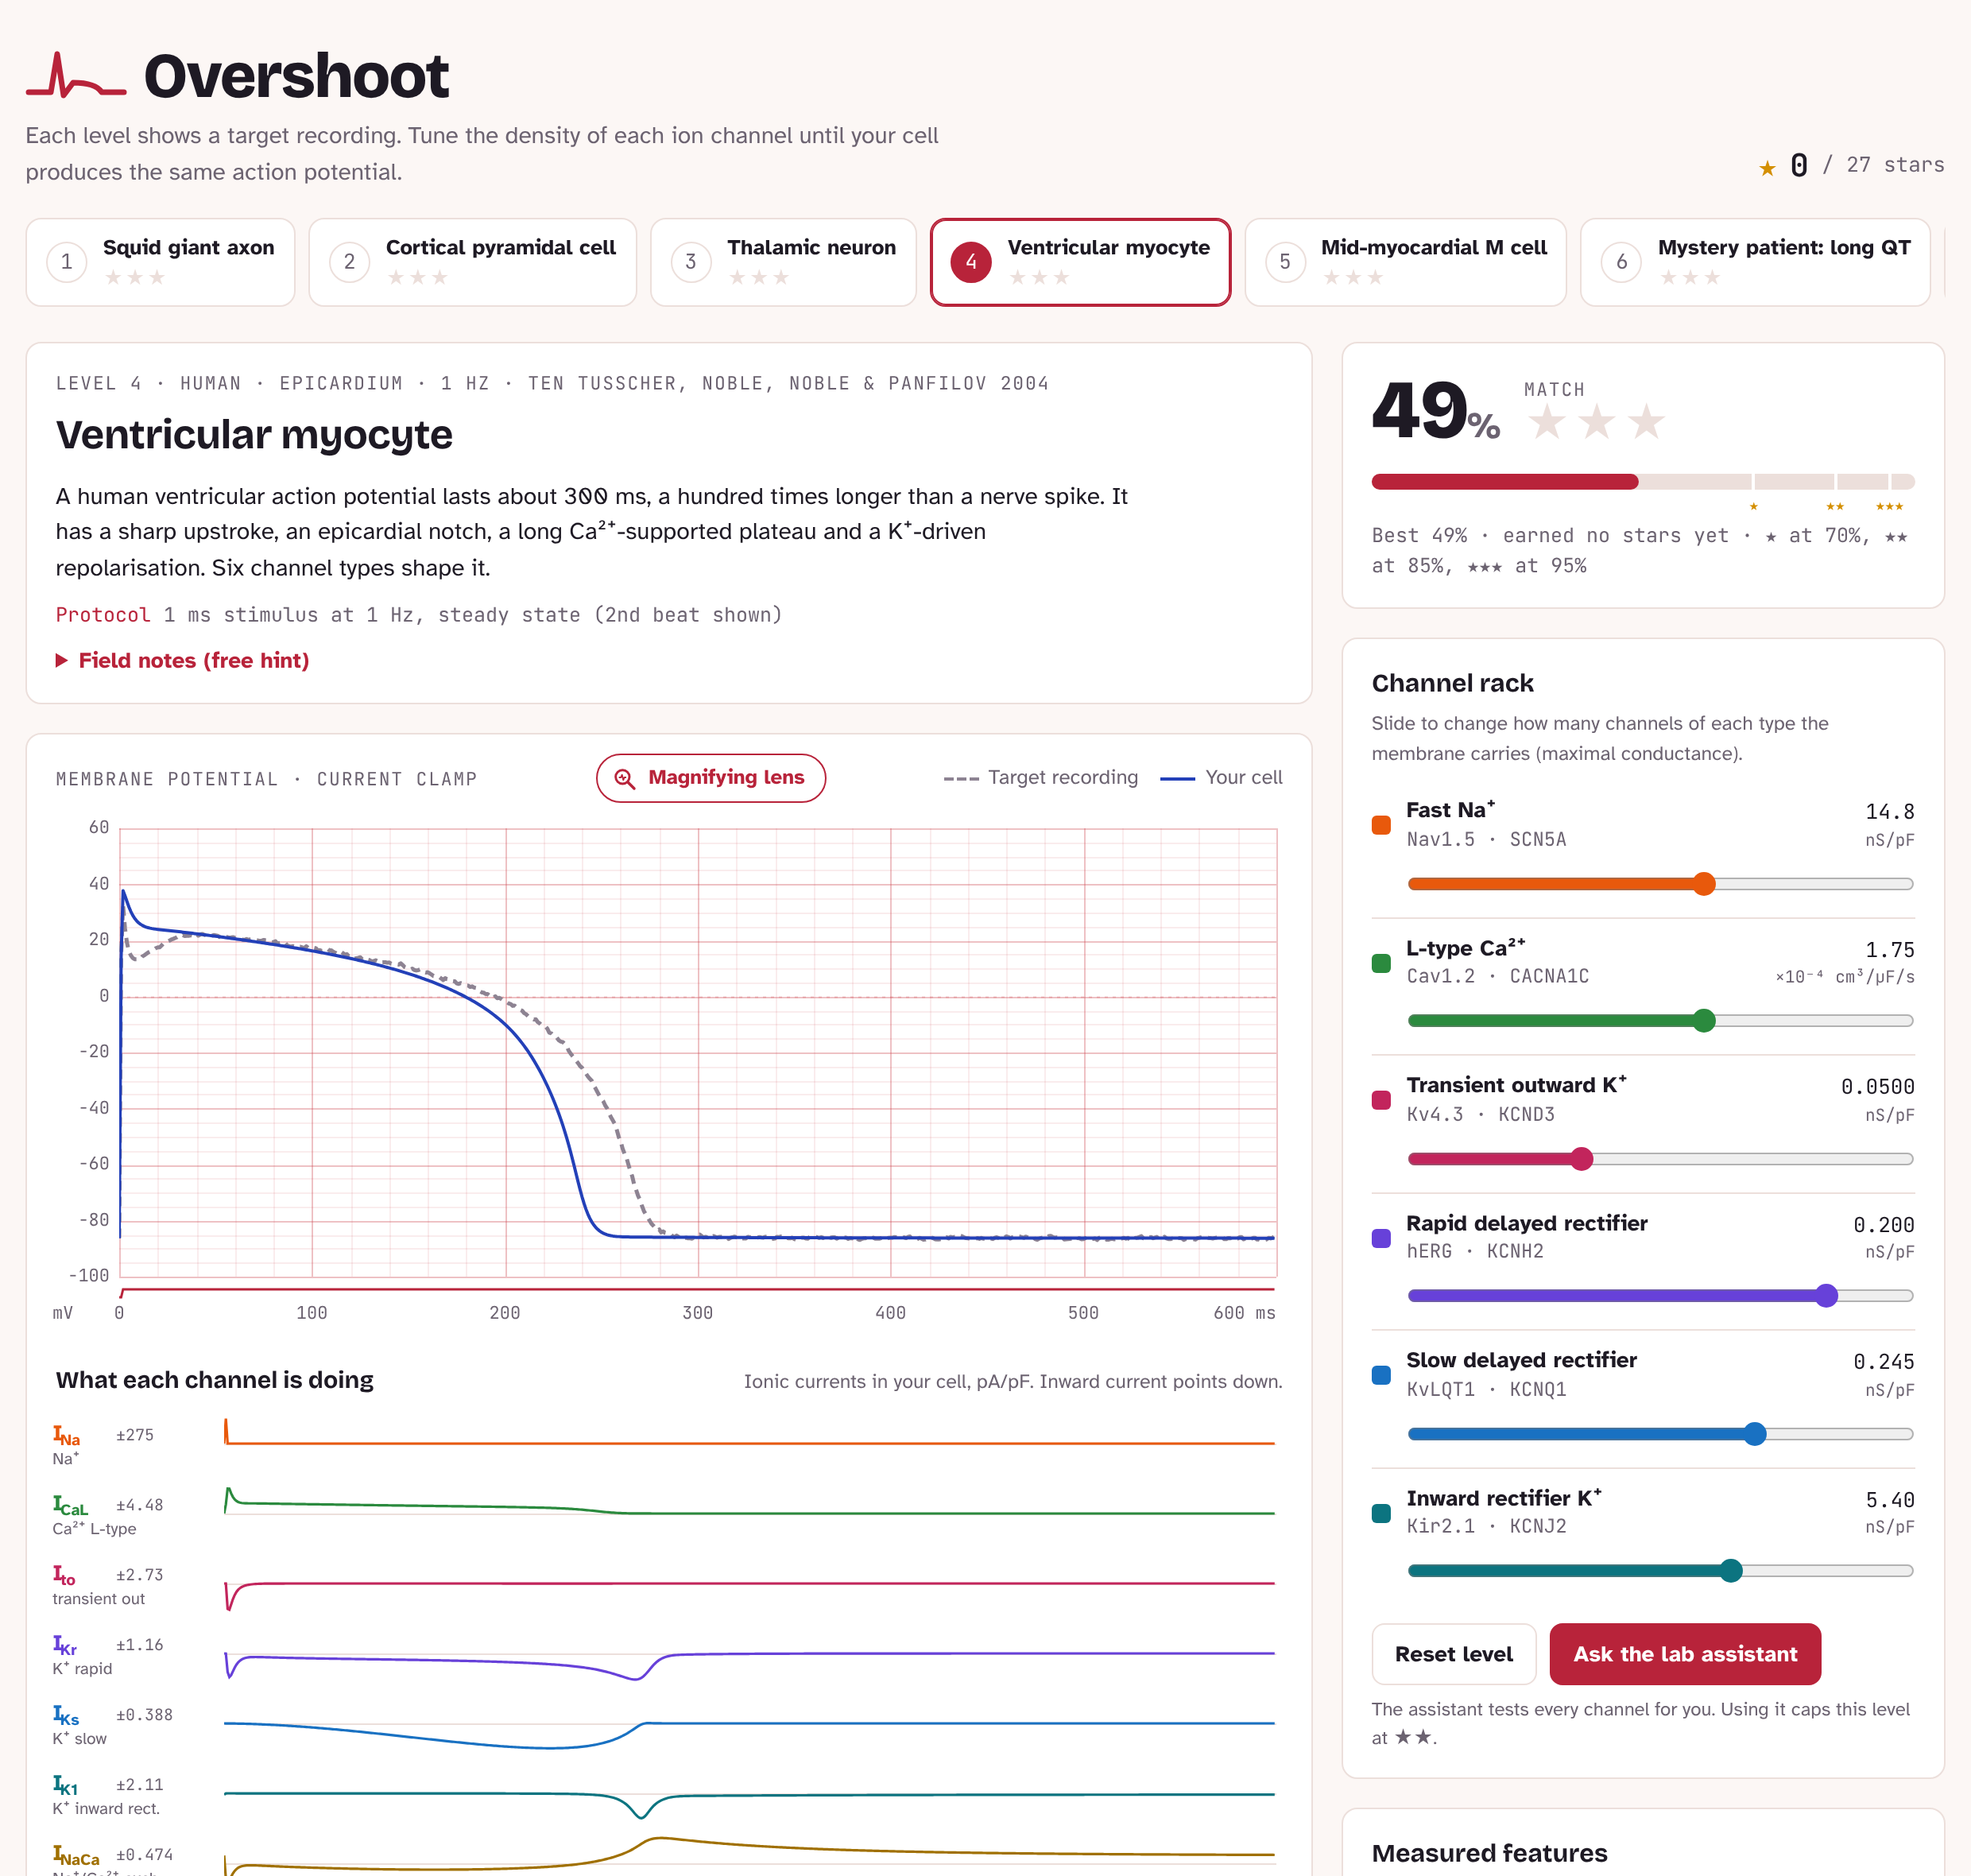
\includegraphics[width=0.95\textwidth]{figures/fig_game.png}
\caption{Level 4 (human epicardial myocyte), partly solved. The target recording (dashed) is drawn on ECG-style paper together with the player's cell (solid). Below are the eight ionic currents (inward current down). On the right are the score, the channel rack (one slider per channel, in physical units, with gene names) and the feature table that explains the score.}
\label{fig:game}
\end{figure}

\paragraph{Scoring like a modeller.} Comparing raw traces point by point punishes a spike train shifted by a millisecond and rewards nothing a physiologist cares about. Overshoot instead extracts electrophysiological features, much as parameter-fitting tools in neuroscience do \cite{VanGeit2016}. Examples are resting potential, overshoot, maximal upstroke velocity, notch depth, action potential duration at 50\% and 90\% repolarisation (APD$_{50}$, APD$_{90}$), spike count, adaptation ratio, burst latency, QRS width, T-wave amplitude, QT interval and T-peak-to-T-end interval. Each feature $f_j$ has a tolerance $\tau_j$ in physical units, and
\begin{equation}
s_j = 100\,\exp\!\left[-\frac{(f_j - f_j^\ast)^2}{2\tau_j^2}\right], \qquad S = \frac{1}{n}\sum_j s_j,
\end{equation}
where $f_j^\ast$ is the target value. For single action potentials, the waveform RMS error is one more feature. Stars are awarded at $S = 70$, 85 and 95\%, the same thresholds on every level. The per-feature bars (figure~\ref{fig:game}, bottom right) tell the player \emph{what} is wrong, which teaches more than a single number.

\paragraph{One idea per level.} The sequence goes from three conductances (squid axon) to slow currents and adaptation \cite{BrownAdams1980}, de-inactivation and rebound bursts, and the phase-by-phase choreography of six cardiac currents. Three applications follow:
\begin{itemize}
\item regional heterogeneity (the M cell);
\item a molecular diagnosis (Timothy syndrome, a gain of function of Cav1.2 \cite{Splawski2004}, approximated as $1.8\times$ the L-type conductance);
\item an electrolyte disorder, in which the tools are extracellular concentrations instead of channel densities.
\end{itemize}
The last two levels move to tissue (section~\ref{sec:ecg}). Figure~\ref{fig:targets} shows four of the targets.

\paragraph{Help, and its price.} A free ``field note'' gives a conceptual hint. A ``lab assistant'' numerically tests modest and large changes of every slider and names the single most useful one. Using it caps the level at two stars. After the first star, a lab-notebook entry explains the physiology and its clinical or historical context. It also compares the player's channel mix with the original model's.

\paragraph{Designed to be identifiable, tested to stay so.} Each level must start clearly wrong but still produce a recognisable waveform. Mystery levels must be solvable only by the right mechanism. Both properties are enforced by automated regression tests:
\begin{itemize}
\item every starting configuration scores below one star;
\item every target scores 100\%;
\item in the long-QT mystery (level 6), no single \emph{wrong} channel reaches one star. Lowering a K$^+$ current lengthens the action potential but cannot raise the plateau, as the extra Ca$^{2+}$ current does.
\end{itemize}
Degeneracy is not hidden; it is the lesson of level 5. The M cell differs from the epicardial cell by a fourfold lower $\IKs$, but some other channel mixes reach a respectable score too \cite{Prinz2004,MarderGoaillard2006}.

\begin{figure}[t]
\centering
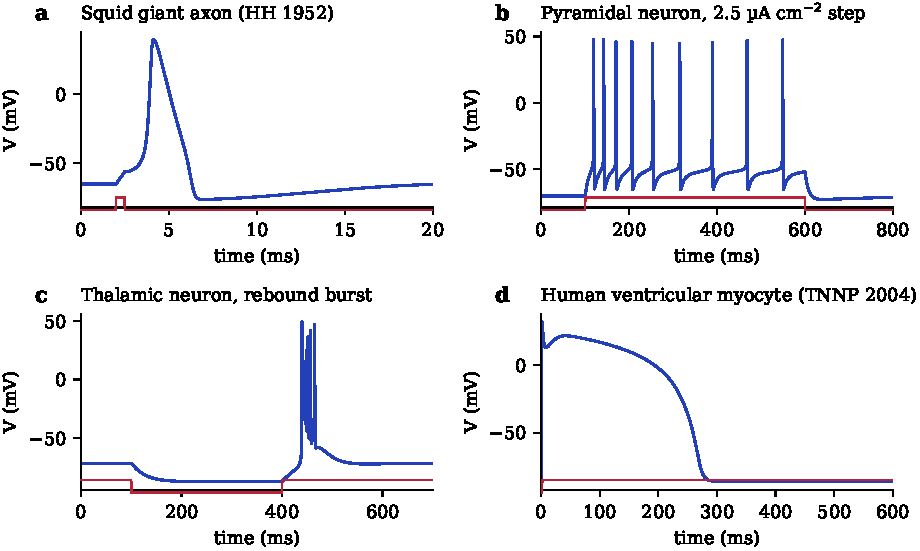
\includegraphics[width=\textwidth]{figures/fig_targets.pdf}
\caption{Target waveforms of four levels, with the stimulus protocol shown as a red trace at the bottom of each panel. (a)~HH squid axon after a \SI{0.5}{\milli\second} shock. (b)~Regular-spiking pyramidal neuron during a \SI{500}{\milli\second} current step; the M-current makes the interspike intervals grow. (c)~Thalamic neuron, rebound burst after release from hyperpolarisation, carried by de-inactivated T-type Ca$^{2+}$ channels. (d)~Human epicardial myocyte at \SI{1}{\hertz}, with its upstroke, notch, plateau and repolarisation.}
\label{fig:targets}
\end{figure}

\section{The magnifying lens: fluxes in physical units}\label{sec:lens}

\begin{figure}[t]
\centering
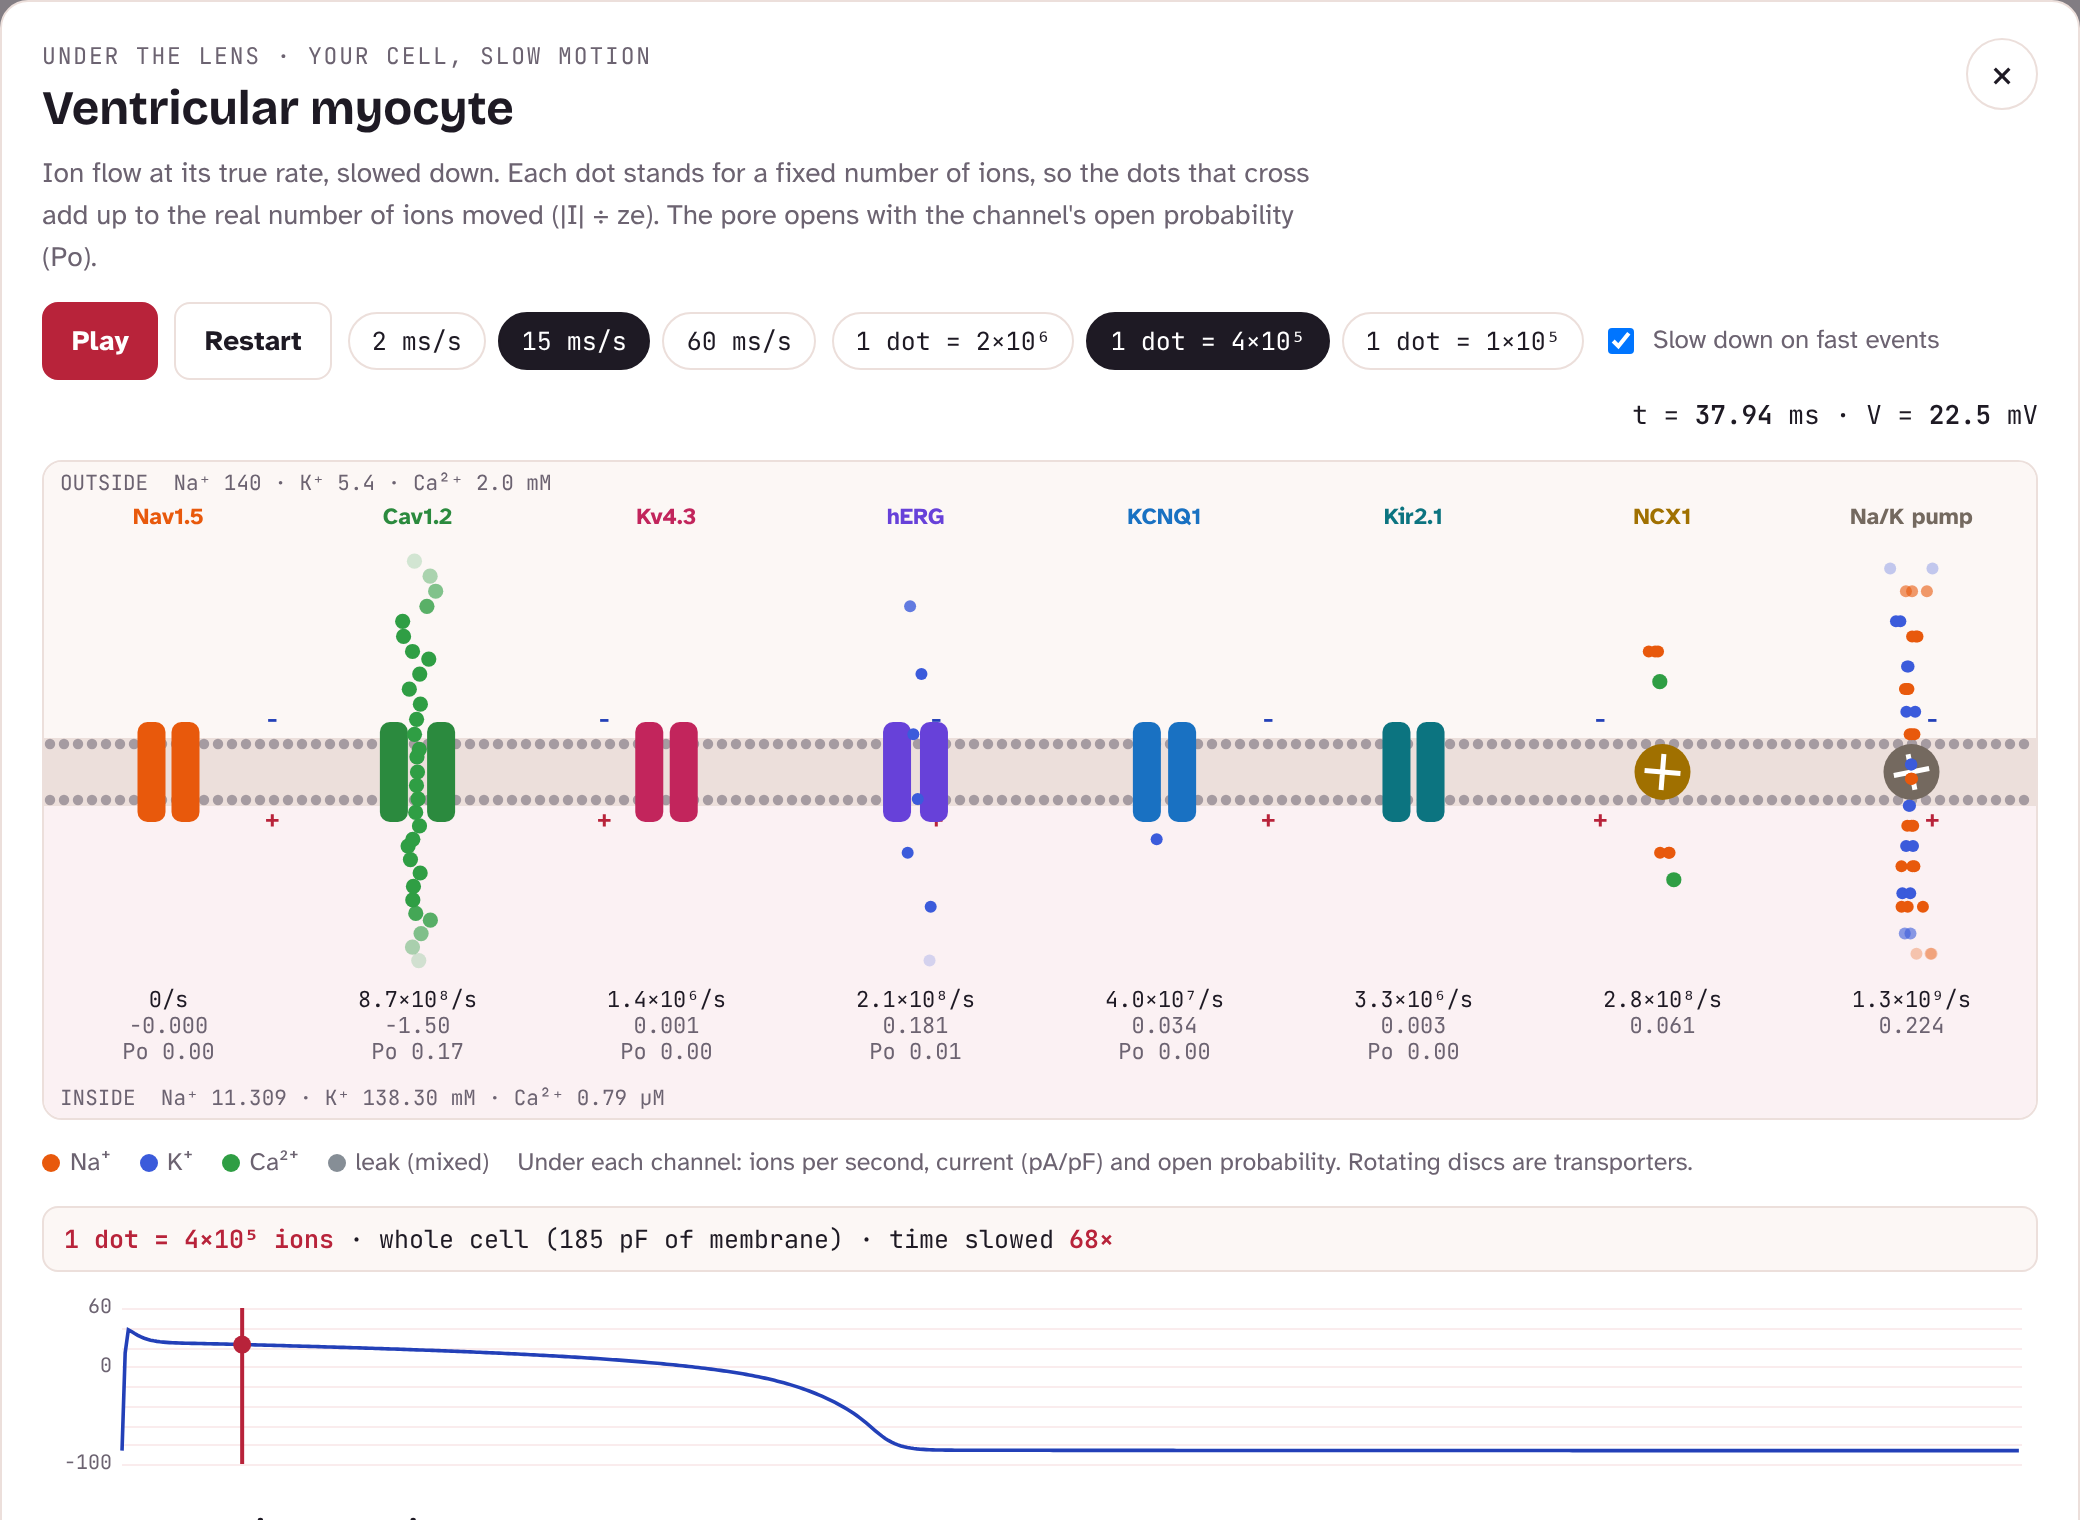
\includegraphics[width=0.92\textwidth]{figures/fig_lens.png}
\caption{The magnifying lens on the epicardial myocyte during the plateau. The pore width of each channel follows its open probability $P_o$. Dots are packets of ions crossing at the calibrated rate of equation~(\ref{eq:dots}). Under each channel are its whole-cell ion flux, current and $P_o$. The bar under the membrane states the ions per dot, the membrane area and the current slow-down factor. Below are $V(t)$ with a scrubbable playhead and the concentration traces.}
\label{fig:lens}
\end{figure}

\begin{figure}[t]
\centering
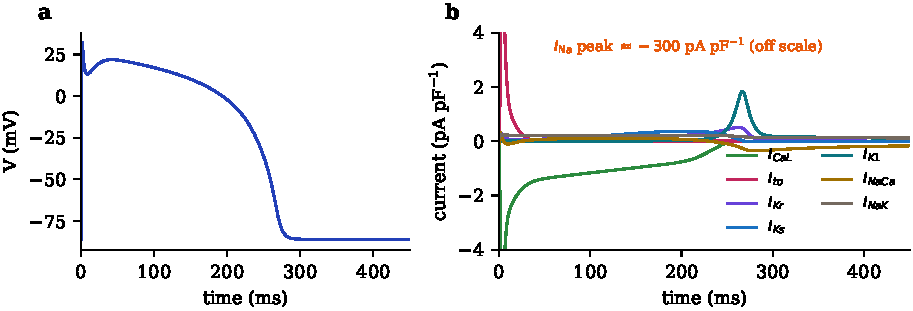
\includegraphics[width=\textwidth]{figures/fig_currents.pdf}
\caption{(a)~Epicardial action potential and (b)~the currents that shape it after the upstroke. The Na$^+$ current is 100 times larger but lasts about \SI{1}{\milli\second}. During the plateau, small inward ($\ICaL$, NCX) and outward ($\IKr$, $\IKs$, pump) currents nearly cancel. This balance is why level~9 works.}
\label{fig:currents}
\end{figure}

A second view replays the player's cell in slow motion (figure~\ref{fig:lens}). Each channel is drawn in a lipid bilayer with a pore whose width follows the open probability, the product of its gates. Coloured dots (Na$^+$, K$^+$, Ca$^{2+}$) cross it in the direction of the current. Rotating discs represent the pump (3 Na$^+$ out, 2 K$^+$ in per cycle) and the exchanger (3 Na$^+$ for 1 Ca$^{2+}$). Plus and minus signs on the two faces of the membrane flip at the overshoot.

The dots are \emph{calibrated}. For a current $I$ carried by an ion of valence $z$ through a membrane of stated area, the flux is $\Phi = |I|/(ze)$. For a transporter carrying one net charge per cycle, $\Phi$ counts all the ions moved per cycle. If one dot represents $N$ ions and playback is slowed so that one second of screen time shows $\kappa$ seconds of cell time, dots are emitted at
\begin{equation}
\dot n_{\mathrm{dots}} = \frac{\kappa\,\Phi}{N}\quad\text{per screen second.}
\label{eq:dots}
\end{equation}
Over any event, the number of dots that cross is $\int \Phi\,\mathrm{d}t / N$, independent of the playback speed. When playback slows down automatically during fast events (the cardiac upstroke lasts about \SI{1}{\milli\second}), the Na$^+$ burst spreads out in screen time but keeps its true size. The value of $N$ is shown at all times. It is chosen so that the busiest current produces a few hundred dots per run, and the player can change it.

We first tried a logarithmic mapping of current to dot rate. It made small currents visible, but it hid exactly what the lens is meant to show: how strongly fluxes change during the action potential. The linear, calibrated mapping keeps that information. It also makes the lens a tool for order-of-magnitude reasoning (section~\ref{sec:class}).

The lens also plots concentrations against time. For the myocyte these are the model's state variables: cytosolic and sarcoplasmic-reticulum Ca$^{2+}$, and the changes in cytosolic Na$^+$ and K$^+$. For the neurons they are estimated by integrating the currents over a stated geometry. For the thalamic cell, a submembrane Ca$^{2+}$ shell is included.

\section{Quantitative checks against physiology}\label{sec:checks}

Because a game invites trust, we checked its key numbers against independent physiological values (table~\ref{tab:checks}). These checks run as automated tests.

\begin{table}[t]
\centering\small
\caption{Model outputs used in the game, compared with independent values where available.}
\label{tab:checks}
\footnotesize
\begin{tabular}{@{}lll@{}}
\toprule
Quantity & Model & Reference value \\
\midrule
HH overshoot / undershoot & \SI{+39}{} / \SI{-76}{\milli\volt} & as published \cite{HH1952} \\
Epicardial APD$_{90}$ at \SI{1}{\hertz} & \SI{271}{\milli\second} & 270--300\,ms in TNNP \cite{TNNP2004} \\
Ca$^{2+}$ entry via $\ICaL$ per beat & $1.7\times10^{8}$ ions $\approx \SI{17}{\micro M}$ cytosol & 10--20\,\si{\micro M} \cite{Bers2002} \\
Cytosolic Ca$^{2+}$ transient & 0.07 $\to$ \SI{0.96}{\micro M} & $\sim$\SI{1}{\micro M} peak \cite{Bers2002} \\
Peak whole-cell Na$^+$ influx & $2.8\times10^{11}$\,s$^{-1}$ for $\sim$\SI{1}{\milli\second} & --- \\
Na$^+$ entry per squid spike (\SI{6.3}{\celsius}) & \SI{14.5}{\pico\mole\per\centi\metre\squared} & minimum $C\Delta V/F = \SI{1.1}{\pico\mole\per\centi\metre\squared}$ \\
Resting potential shift, $[\mathrm{K}^+]_o$ 5.4 $\to$ \SI{8}{\milli M} & \SI{10.3}{\milli\volt} & Nernst: \SI{10.5}{\milli\volt} \\
\bottomrule
\end{tabular}
\end{table}

\section{From cell to ECG}\label{sec:ecg}

\paragraph{Level 8: the T wave.} The player starts from a \emph{uniform} wall and finds a QRS that is too narrow and a T wave that points the wrong way (figure~\ref{fig:ecg}a, grey). This is the textbook expectation. If every cell had the same action potential duration, the cells activated last would also repolarise last. The repolarisation gradient would then have the same sign as the activation gradient, and in equation~(\ref{eq:pseudoecg}) a recovery wave travelling in the same direction contributes with the opposite sign. Real hearts reverse this order with a transmural gradient of K$^+$ channels \cite{YanAntzelevitch1998}. The epicardium, activated last, has the shortest action potential, and the mid-myocardial M cells the longest (figure~\ref{fig:ecg}b).

One modelling choice needed care. With TNNP 2004's uniform $\IKs$ (\SI{0.245}{\nano\siemens\per\pico\farad}) and a realistic transmural conduction velocity of about \SI{46}{\centi\metre\per\second} ($D = \SI{7e-4}{\centi\metre\squared\per\milli\second}$), the activation delay across the wall exceeds the endo--epi difference in action potential duration. The T wave then stays inverted. Using the epicardial $\IKs$ of the 2006 revision of the model (\SI{0.392}{\nano\siemens\per\pico\farad}) \cite{TP2006} gives an upright T wave with amplitude 0.21 relative to the QRS, a \SI{26}{\milli\second} QRS and a QT of \SI{296}{\milli\second}. Halving the gap-junction coupling widens the QRS by more than \SI{5}{\milli\second}, which the tests check.

\paragraph{Level 9: the hERG paradox.} Block of the hERG channel ($\IKr$) is the classic cause of drug-induced long QT and torsade de pointes \cite{SanguinettiTF2006,Redfern2003}. In level 9, a compound blocks 60\% of hERG current, fixed as if measured in a patch-clamp screen, yet the ``trial'' ECG shows a nearly normal QT. hERG block alone lengthens QT from 296 to \SI{322}{\milli\second}. Adding 30\% block of the L-type Ca$^{2+}$ channel restores \SI{294}{\milli\second} (figure~\ref{fig:ecg}c). This is the verapamil pattern \cite{Zhang1999}, and it is part of the motivation for the CiPA initiative, which combines several channel assays with a human ventricular model \cite{Colatsky2016,OHara2011}. The sliders in this level can only \emph{block}, between 5\% and 100\% of control current. An earlier draft allowed values above 100\%, and a 50\% increase of $\IKs$ then scored one star by the wrong mechanism.

\begin{figure}[t]
\centering
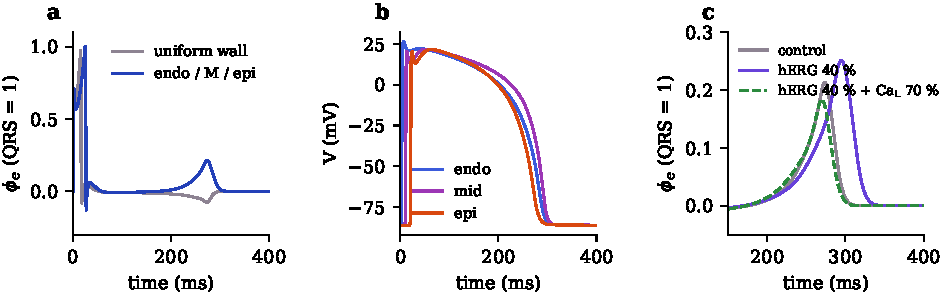
\includegraphics[width=\textwidth]{figures/fig_ecg.pdf}
\caption{Pseudo-ECGs from the transmural strand. (a)~A uniform wall gives a narrow QRS and an inverted T wave. Endocardial, M and epicardial layers give a wider QRS and an upright T wave. (b)~Action potentials at mid-depth of each layer in the layered wall: the epicardium is activated last and repolarises first. (c)~T waves for a control wall, 60\% hERG block, and 60\% hERG block plus 30\% L-type Ca$^{2+}$ block.}
\label{fig:ecg}
\end{figure}

\section{Classroom use}\label{sec:class}

Overshoot can be played on its own, and it supports short quantitative exercises that connect the game to undergraduate physics.
\begin{enumerate}
\item \textbf{Nernst in action.} In level 7, predict the resting-potential shift for $[\mathrm{K}^+]_o = 5.4 \to \SI{8}{\milli M}$ from $E_K = (RT/F)\ln([\mathrm{K}^+]_o/[\mathrm{K}^+]_i)$, then measure it in the game (table~\ref{tab:checks}). Explain the small residual using the other currents in equation~(\ref{eq:membrane}).
\item \textbf{Charge versus concentration.} Using the lens on level 1, compare the Na$^+$ entering per spike with the minimum charge needed to charge the membrane, $C_m\Delta V \approx \SI{0.1}{\micro\coulomb\per\centi\metre\squared}$, i.e.\ about \SI{1}{\pico\mole\per\centi\metre\squared}. Why does the model, like real squid axons \cite{KeynesLewis1951}, let in several times more? (Hint: overlap of Na$^+$ and K$^+$ currents \cite{CarterBean2009,Alle2009}.) Then estimate how many spikes a \SI{0.5}{\milli\metre} axon could fire before its internal Na$^+$ rose by 10\%.
\item \textbf{Degeneracy.} In level 5, find two visibly different channel mixes with $S > 85\%$. Which extra protocol would tell them apart: a different pacing rate, or a drug?
\item \textbf{Dipoles and the T wave.} Using equation~(\ref{eq:pseudoecg}), sketch the sign of $\phi_e$ for an activation front and for a repolarisation front moving towards the electrode, and predict the T-wave polarity of a uniform wall before playing level 8.
\item \textbf{Calibration.} From the lens readout, verify that the number of dots crossing during the cardiac upstroke times $N$ equals $\int \Phi\,\mathrm{d}t$, and that it does not change with playback speed.
\end{enumerate}

\section{Limitations}\label{sec:limits}

\begin{itemize}
\item \textbf{Simplified tissue.} The ECG levels use a one-dimensional strand. The real QRS also depends on the three-dimensional activation sequence set by the Purkinje network, on the heart's geometry and on the torso. The level debrief says so.
\item \textbf{Modelling approximations.} Intracellular Na$^+$ and K$^+$ are held fixed during play. Timothy syndrome is approximated as a conductance increase, whereas the real mutation mainly impairs inactivation \cite{Splawski2004}. TNNP 2004 is less sensitive to $\IKr$ than later human models \cite{OHara2011}, so hERG effects are smaller than in the clinic.
\item \textbf{Levels that were rejected.} We prototyped hyperkalaemia and Brugada-syndrome ECG levels and rejected both, because the model did not reproduce the clinical picture. The T wave shrank instead of peaking, and the epicardial plateau never collapsed. We follow a simple rule: a level is built only if the model reproduces the clinical picture. A newer model may allow these levels.
\item \textbf{No classroom evaluation yet.} We have not yet measured learning gains. A pre/post concept inventory on membrane biophysics is the natural next step.
\end{itemize}

\section{Conclusions}

Overshoot presents conductance-based membrane models as an inverse problem that students can play. The targets are published physiology, the controls are channel densities and ion concentrations in physical units, and the score is a feature-based fit. One self-contained HTML file covers a path from the squid axon to the T wave and a drug-safety argument. Because the source is open and the levels are defined declaratively, instructors can add levels for their own courses.

\section*{Acknowledgements}
The game's code and a first draft of this manuscript were written with the assistance of an AI model (Claude, Anthropic), under the author's direction. All model outputs reported here are reproduced by scripts in the repository.

\bibliographystyle{iopart-num}
\bibliography{refs}

\end{document}
